\documentclass{article}

\usepackage[english]{babel}
\usepackage[
    a4paper,
    top=2cm,
    bottom=2cm,
    left=3cm,
    right=3cm,
    marginparwidth=1.75cm
]{geometry}
\usepackage{amsmath}
\usepackage{graphicx}
\usepackage{xcolor}
\usepackage[colorlinks=true, allcolors=blue]{hyperref}
\usepackage{placeins}
\usepackage{subcaption}
\usepackage{listings}
\usepackage{indentfirst}

\setlength{\parindent}{0.2in}
\setlength{\parskip}{5pt}

\lstset{ language=Python, basicstyle=\ttfamily\footnotesize, keywordstyle=
\color{blue!80!black}
\bfseries, commentstyle=
\color{green!60!black}
\itshape, stringstyle=
\color{orange!90!black}
, identifierstyle=
\color{black}
, emphstyle=
\color{purple!80!black}
\bfseries, numbers=left, numberstyle=\tiny
\color{gray!60}
, stepnumber=1, numbersep=10pt, tabsize=4, breaklines=true, breakatwhitespace=true,
frame=none, backgroundcolor=
\color{gray!8}
, showstringspaces=false, captionpos=b, xleftmargin=15pt, xrightmargin=5pt,
aboveskip=12pt, belowskip=12pt, lineskip=0.8pt, moredelim=[s][
\color{orange!90!black}
]{'''}{'''}, moredelim=[s][
\color{orange!90!black}
]{"""}{"""}, literate={0}{{{\color{purple!80!black}0}}}1 {1}{{{\color{purple!80!black}1}}}1
{2}{{{\color{purple!80!black}2}}}1 {3}{{{\color{purple!80!black}3}}}1 {4}{{{\color{purple!80!black}4}}}1
{5}{{{\color{purple!80!black}5}}}1 {6}{{{\color{purple!80!black}6}}}1 {7}{{{\color{purple!80!black}7}}}1
{8}{{{\color{purple!80!black}8}}}1 {9}{{{\color{purple!80!black}9}}}1 }
\graphicspath{{Images/}}
\title{\textbf{PUNCH!}}
\author{Kim Hyeong-Seok}
\begin{document}
    \maketitle
    \begin{abstract}
        PUNCH! is a mobile application designed to facilitate combat-style
        exercise using only a smartphone, enabling users to engage in physical activity
        even in confined spaces. This paper details the development and testing
        of PUNCH!, focusing on the utilization of smartphone sensors to track
        movement and classify punch types. The application employs advanced techniques
        such as orientation estimation, noise reduction, and deep learning models
        to achieve accurate motion detection and classification. The results
        demonstrate the feasibility of using smartphones for effective combat-style
        exercise, addressing common barriers to physical activity in modern lifestyles.
    \end{abstract}

    \section{Introduction}
    Modern individuals often struggle to maintain a healthy lifestyle due to a
    lack of physical activity, chronic stress, and the demands of a busy daily
    routine. In particular, time and space constraints, financial burdens, and
    psychological barriers associated with exercise contribute to the growing
    difficulty of engaging in regular physical activity. To address these challenges,
    we developed PUNCH!, a mobile application that enables users to easily
    engage in combat-style exercise using only a smartphone, even within confined
    spaces.

    The development and testing of this application were conducted using a MacBook
    Pro (M1, 2021) and an iPhone 14 Pro, which will hereafter be referred to as the
    smartphone. All data collection and code execution were performed
    exclusively on these two devices, and the application has not been tested on
    platforms other than iOS.
    \section{Methods}
    \subsection{Utilization of Smartphone Sensors}
    \subsubsection{Measurement of Acceleration via Calibration and Differencing}
    To isolate acceleration caused solely by device movement, a calibration process
    was performed by maintaining the smartphone in a standard orientation—perpendicular
    to the ground with the screen facing the user—for one second. The
    accelerometer readings obtained during this calibration were used as a
    reference, and subsequent acceleration measurements were compared against this
    baseline to estimate changes due exclusively to motion. This approach
    assumes gravitational acceleration as a constant bias, allowing for a simplified
    implementation that focuses on relative changes in acceleration.

    However, gravitational force continuously affects accelerometer readings, and
    variations in device tilt or orientation can significantly alter the measured
    values. As such, ignoring the influence of gravity imposes a limitation on the
    accuracy of this method. The approach lacks the precision necessary to
    isolate pure translational acceleration. Consequently, we decided to
    incorporate a mathematically and physically grounded method for tracking the
    device’s orientation to account for gravitational effects more accurately. \FloatBarrier
    \begin{figure}
        \centering
        \includegraphics[width=\textwidth]{
            Images/data_difference_and_integration.png
        }
        \caption{Charts comparing raw data and differentiated data}
        \label{fig:data_difference_and_integration}
        \centering
        \includegraphics[width=\textwidth]{Images/error_3d_path.png}
        \caption{An image of 3-dimension path estimated with differentiated data}
        \label{fig:error_3d_path}
    \end{figure}

    \FloatBarrier
    \subsubsection{Orientation Estimation Using the Accelerometer}

    \FloatBarrier
    \begin{figure}[ht]
        \centering
        \includegraphics[width=7.5cm]{Images/accelerometer.png}
        \caption{Smartphone accelerometer axis orientation}
        \label{fig:accelerometer}
    \end{figure}

    The coordinate system of the smartphone's accelerometer follows the right-hand
    rule, as illustrated in Figure~\ref{fig:accelerometer}. The output values of
    the sensor are normalized by the gravitational acceleration
    $9.8\,\mathrm{m/s^2}$, and thus each axis returns a value in units of $g$ (an
    equivalent to gravitational force).

    When the smartphone is held vertically such that the $xz$-plane is parallel to
    the ground and the screen is facing the user, the expected accelerometer
    reading $\vec{g}$ due to gravity is:

    \[
        \vec{g}=
        \begin{bmatrix}
            0 & -1 & 0
        \end{bmatrix}^{\top}
    \]

    This vector $\vec{g}$ serves as the reference vector, representing the
    direction of gravity in the device's coordinate system under ideal upright
    conditions.

    Let $\begin{bmatrix}
        x & y & z
    \end{bmatrix}^{\top}$ be the first accelerometer reading obtained after
    calibration. By comparing this measurement to the reference vector, we can
    estimate the initial orientation of the device. Before doing so, the
    accelerometer vector must be normalized to ensure consistency in magnitude.

    The orientation is estimated using a sequence of rotation matrices about the
    $x$-, $y$-, and $z$-axes:

    \[
        R_{x}(\theta_{x}) =
        \begin{bmatrix}
            1 & 0              & 0               \\
            0 & \cos\theta_{x} & -\sin\theta_{x} \\
            0 & \sin\theta_{x} & \cos\theta_{x}
        \end{bmatrix}
    \]
    \[
        R_{y}(\theta_{y}) =
        \begin{bmatrix}
            \cos\theta_{y}  & 0 & \sin\theta_{y} \\
            0               & 1 & 0              \\
            -\sin\theta_{y} & 0 & \cos\theta_{y}
        \end{bmatrix}
    \]
    \[
        R_{z}(\theta_{z}) =
        \begin{bmatrix}
            \cos\theta_{z} & -\sin\theta_{z} & 0 \\
            \sin\theta_{z} & \cos\theta_{z}  & 0 \\
            0              & 0               & 1
        \end{bmatrix}
    \]

    Assuming that the orientation angles $\theta_{x}$, $\theta_{y}$, and $\theta_{z}$
    represent rotations about the respective axes, the rotated reference vector
    becomes:

    \[
        \begin{bmatrix}
            x \\
            y \\
            z
        \end{bmatrix}
        = R_{y}(\theta_{y}) \cdot R_{x}(\theta_{x}) \cdot R_{z}(\theta_{z}) \cdot
        \begin{bmatrix}
            0  \\
            -1 \\
            0
        \end{bmatrix}
        = R_{y}(\theta_{y}) \cdot R_{x}(\theta_{x}) \cdot
        \begin{bmatrix}
            \sin\theta_{z}  \\
            -\cos\theta_{z} \\
            0
        \end{bmatrix}
        = R_{y}(\theta_{y}) \cdot
        \begin{bmatrix}
            \sin\theta_{z}                \\
            -\cos\theta_{x}\cos\theta_{z} \\
            -\sin\theta_{x}\cos\theta_{z}
        \end{bmatrix}
    \]

    Multiplying out the rotations yields:

    \[
        \begin{bmatrix}
            x \\
            y \\
            z
        \end{bmatrix}
        =
        \begin{bmatrix}
            \cos\theta_{y}\sin\theta_{z}- \sin\theta_{x}\sin\theta_{y}\cos\theta_{z}  \\
            -\cos\theta_{x}\cos\theta_{z}                                             \\
            -\sin\theta_{y}\sin\theta_{z}- \sin\theta_{x}\cos\theta_{y}\cos\theta_{z}
        \end{bmatrix}
    \]

    Since the accelerometer cannot determine rotation about the $y$-axis (yaw), we
    assume $\theta_{y}= 0$, simplifying the expression to:

    \[
        \begin{bmatrix}
            x \\
            y \\
            z
        \end{bmatrix}
        =
        \begin{bmatrix}
            \sin\theta_{z}                \\
            -\cos\theta_{x}\cos\theta_{z} \\
            -\sin\theta_{x}\cos\theta_{z}
        \end{bmatrix}
    \]

    From this simplified form, we can compute the orientation angles as follows.
    The $x$-component yields:

    \[
        \theta_{z}= \arcsin(x)
    \]

    To isolate $\theta_{x}$, we divide the third component by the second:

    \[
        \frac{z}{y}= \frac{-\sin\theta_{x}\cos\theta_{z}}{-\cos\theta_{x}\cos\theta_{z}}
        = \tan\theta_{x}\quad \Rightarrow \quad \theta_{x}= \arctan\left(\frac{z}{y}
        \right)
    \]

    Let the initial orientation of the device be denoted by $\begin{bmatrix}
        \psi_{0} & \theta_{0} & \phi_{0}
    \end{bmatrix}^{\top}$, corresponding to rotations around the $x$-, $y$-, and
    $z$-axes, respectively. Using the above method, we can estimate the initial
    orientation as:

    \[
        \begin{bmatrix}
            \psi_{0}   \\
            \theta_{0} \\
            \phi_{0}
        \end{bmatrix}
        =
        \begin{bmatrix}
            \arctan\left(\frac{z}{y}\right) \\
            0                               \\
            \arcsin(x)
        \end{bmatrix}
    \]

    This method allows for a simple and effective estimation of the device’s initial
    pitch and roll, based on gravitational acceleration and assuming no initial
    yaw rotation.

    \begin{lstlisting}[language=Python, caption={Orientation estimation using accelerometer data}, label={lst:orientation_estimation}]
def numerical_integration_with_range(self, integrand, start, end):
    result = [0.0]
    for idx, i in enumerate(range(start + 1, end + 1)):
        result.append((integrand[i] + integrand[i - 1]) * (self.time[i] - self.time[i - 1]) / 2 + result[idx - 1])
    return result

def initialize_orientation(self):
    _initial_vector = np.array([self.acceleration_x[0], self.acceleration_y[0], self.acceleration_z[0]])
    _initial_vector = _initial_vector / np.linalg.norm(_initial_vector)
    
    self.initial_rotation_x = np.arctan2(_initial_vector[2], _initial_vector[1])
    self.initial_rotation_y = 0.0
    self.initial_rotation_z = np.arcsin(_initial_vector[0])
    
    print(f"Initial Vector: {_initial_vector}")
    print(f"Initial Rotation: {np.degrees(self.initial_rotation_x)}, {np.degrees(self.initial_rotation_y)}, {np.degrees(self.initial_rotation_z)}")
    
    self.rotation_x = [p + self.initial_rotation_x for p in self.numerical_integration(self.gyro_x, self.time)]
    self.rotation_y = [r + self.initial_rotation_y for r in self.numerical_integration(self.gyro_y, self.time)]
    self.rotation_z = [y + self.initial_rotation_z for y in self.numerical_integration(self.gyro_z, self.time)]
\end{lstlisting}

    \subsubsection{Valid Range for Accelerometer-Based Orientation Estimation}

    When the smartphone is tilted around the $z$-axis, the $x$-axis acceleration
    value increases, while the $y$ and $z$ acceleration values approach zero. In
    this case, the term $z \div y$ in the previous orientation estimation
    formula diverges, leading to instability in the computation of $\theta_{x}$.

    To address this issue, an alternative derivation using a product of the $y$
    and $z$ components is proposed. Starting from the simplified rotation matrix:

    \[
        x = \sin\theta_{z}
    \]
    \[
        y \cdot z = \cos\theta_{x}\cos\theta_{z}\sin\theta_{x}\cos\theta_{z}= \sin
        \theta_{x}\cos\theta_{x}\cos^{2}\theta_{z}= \sin\theta_{x}\cos\theta_{x}(
        1 - \sin^{2}\theta_{z}) = \frac{1}{2}\sin(2\theta_{x}) (1 - x^{2})
    \]

    From this, we can isolate $\theta_{x}$ as:

    \[
        \theta_{x}= \frac{1}{2}\arcsin\left(\frac{y \cdot z}{1 - x^{2}}\right)
    \]

    However, this formulation also fails when the $x$-axis acceleration value approaches
    $1$ or $-1$, i.e., when $\theta_{z}\rightarrow \pm \frac{\pi}{2}$, which corresponds
    to tilting the smartphone to 90 degrees around the $z$-axis. In this
    situation, the denominator $1 - x^{2}$ approaches zero, causing the
    expression to diverge and leading to instability in the calculation of
    $\theta_{x}$.

    Empirical tests showed that when the tilt angle exceeds approximately
    $80^{\circ}$, the accelerometer data becomes increasingly noisy and unreliable,
    as illustrated in Figure~\ref{fig:valid_range_test}. In such cases, the
    estimated $\theta_{x}$ value becomes extremely large and physically
    implausible.

    To ensure reliable orientation estimation, we restrict the accelerometer-based
    calculation of orientation (Section~2.1.2) to cases where the cosine
    similarity between the reference vector $\vec{g}$ and the normalized
    acceleration vector $\mathbf{a}$ is greater than $0.5$, which corresponds to
    a maximum tilt angle of approximately $60^{\circ}$ from the ideal upright orientation:

    \[
        \cos\theta = \frac{ \vec{g} \cdot \vec{a}}{\| \vec{g}\| \|\vec{a}\|}= \frac{-a_{y}}{\|\vec{a}\|}
        > 0.5
    \]

    If the initial orientation does not satisfy this condition, the user is prompted
    to hold the device in an upright position to proceed with calibration.

    \FloatBarrier
    \begin{figure}[ht]
        \centering
        \begin{subfigure}
            {0.48\textwidth}
            \centering
            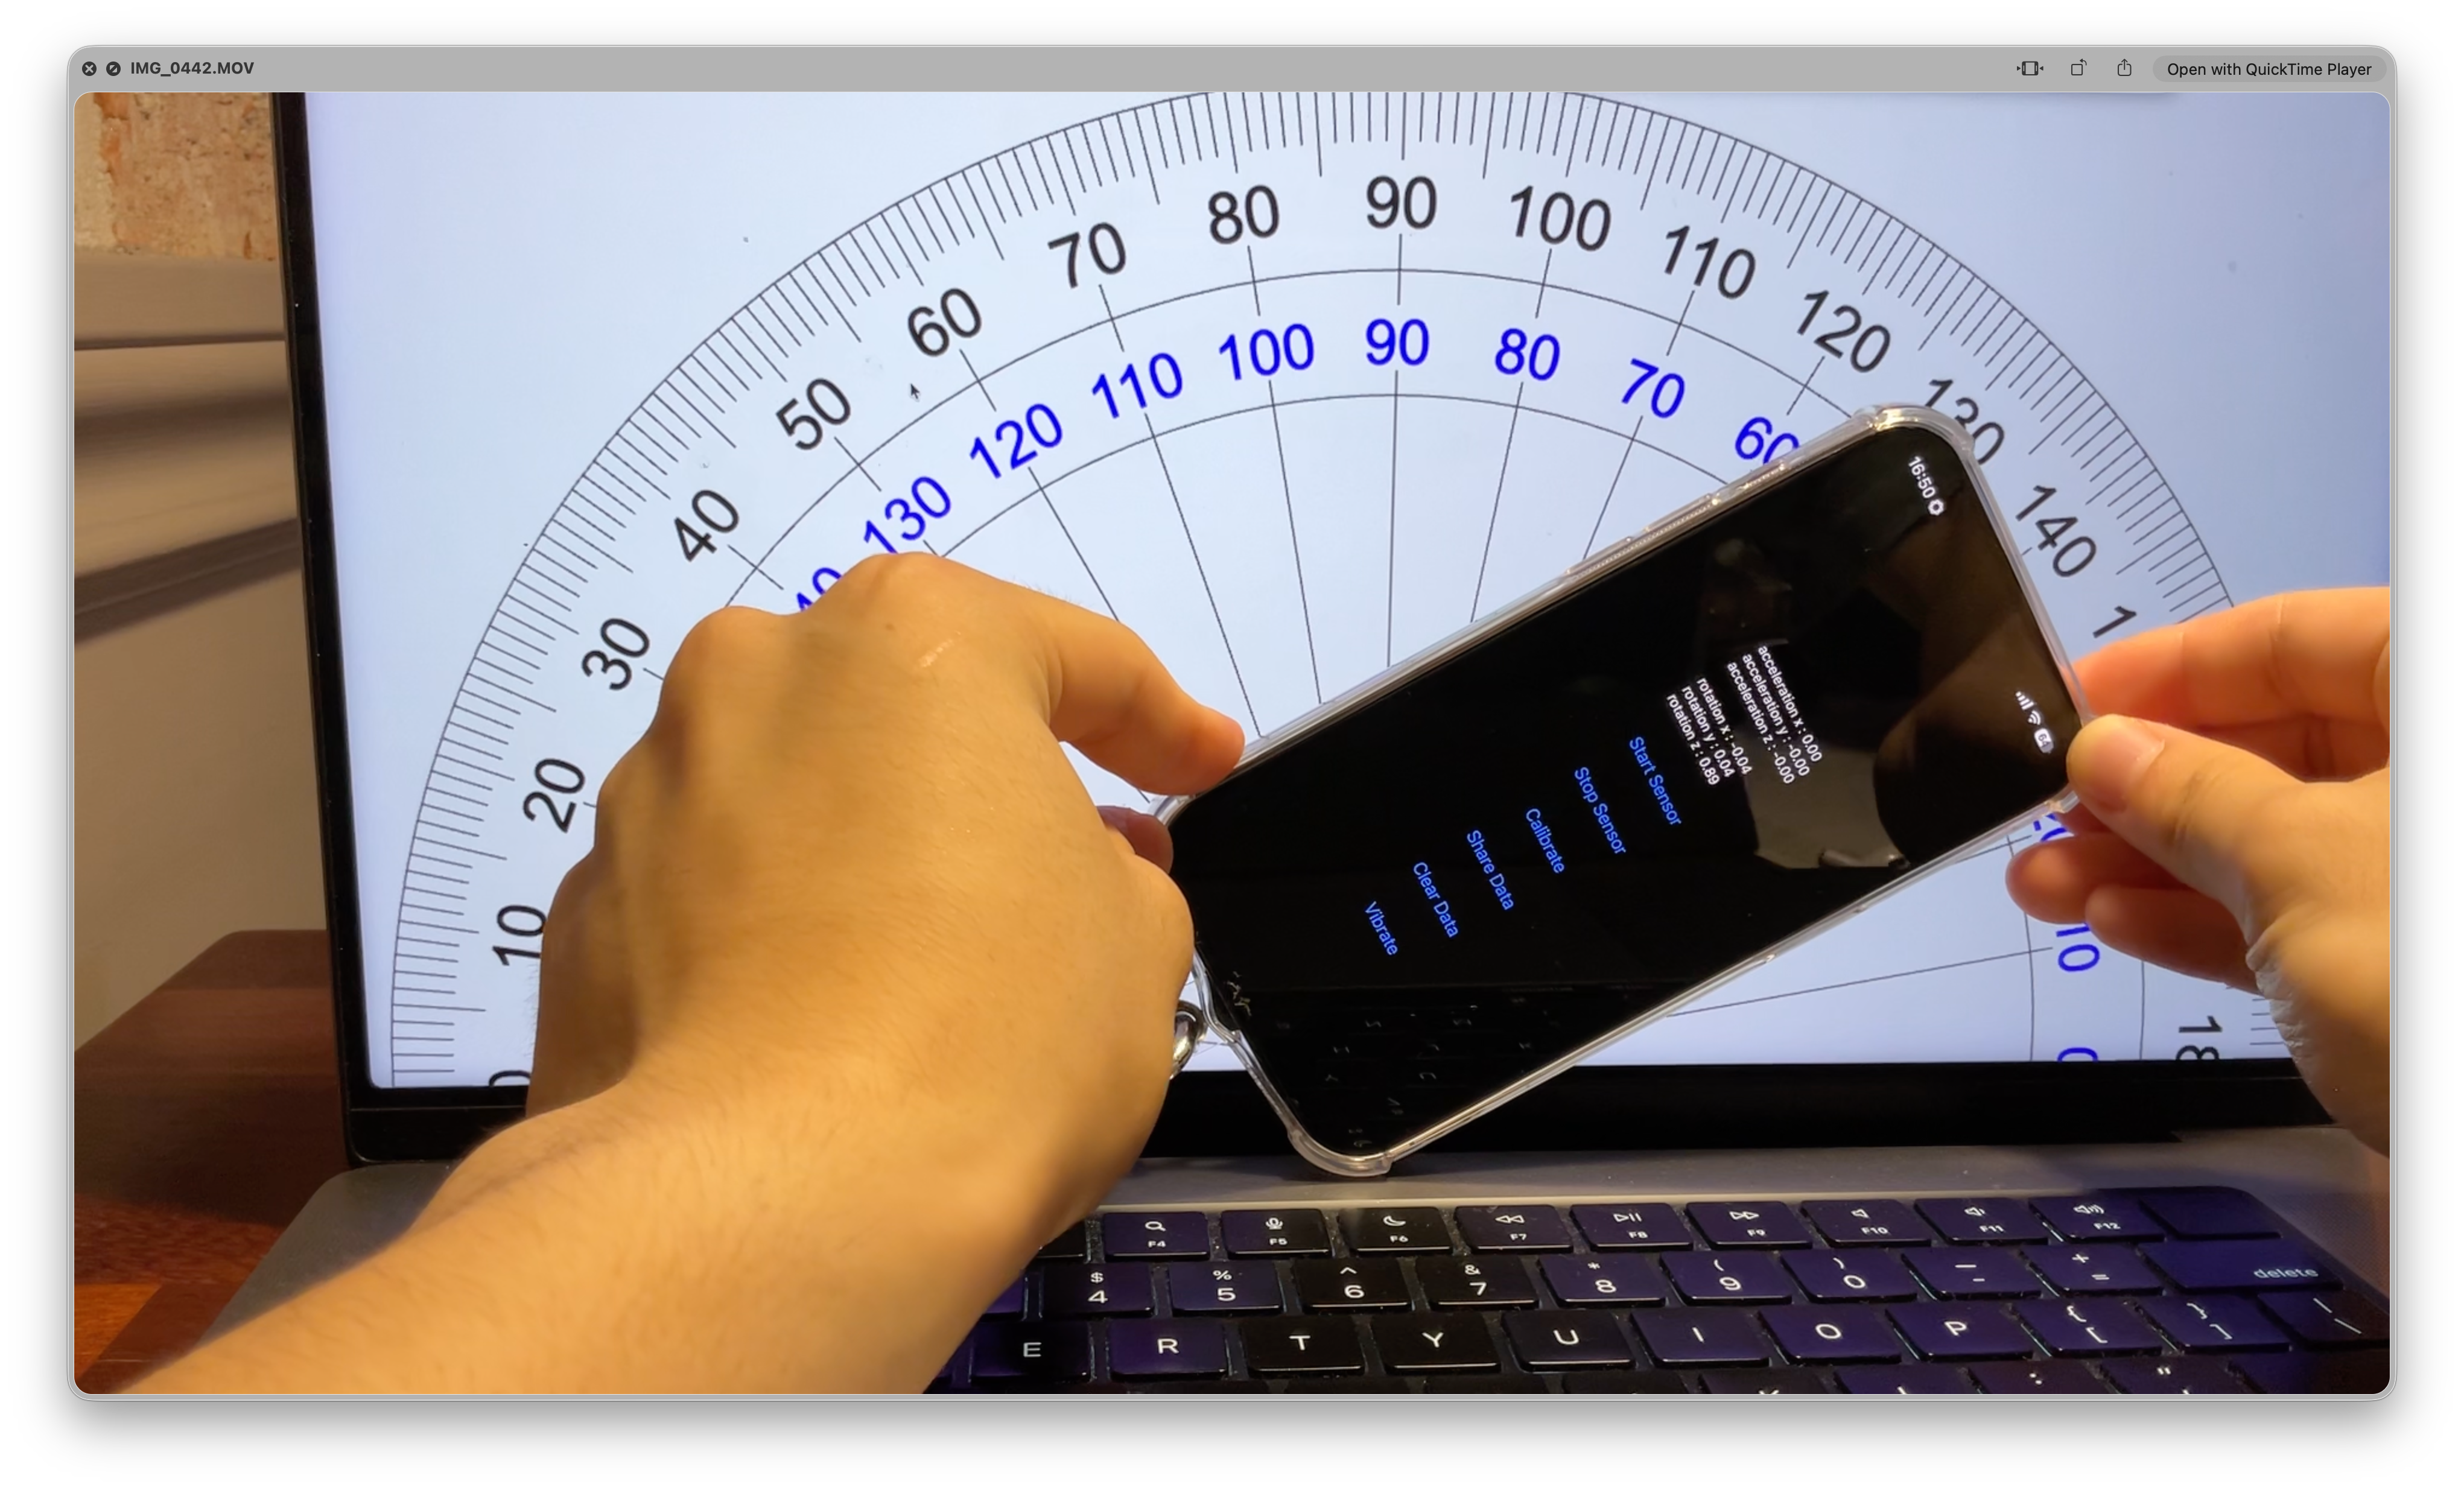
\includegraphics[width=0.9\textwidth]{Images/2_1_3_1.jpg}
            \caption{An image of appropriately estimated orientation}
            \label{fig:2_1_3_1}
        \end{subfigure}
        \begin{subfigure}
            {0.48\textwidth}
            \centering
            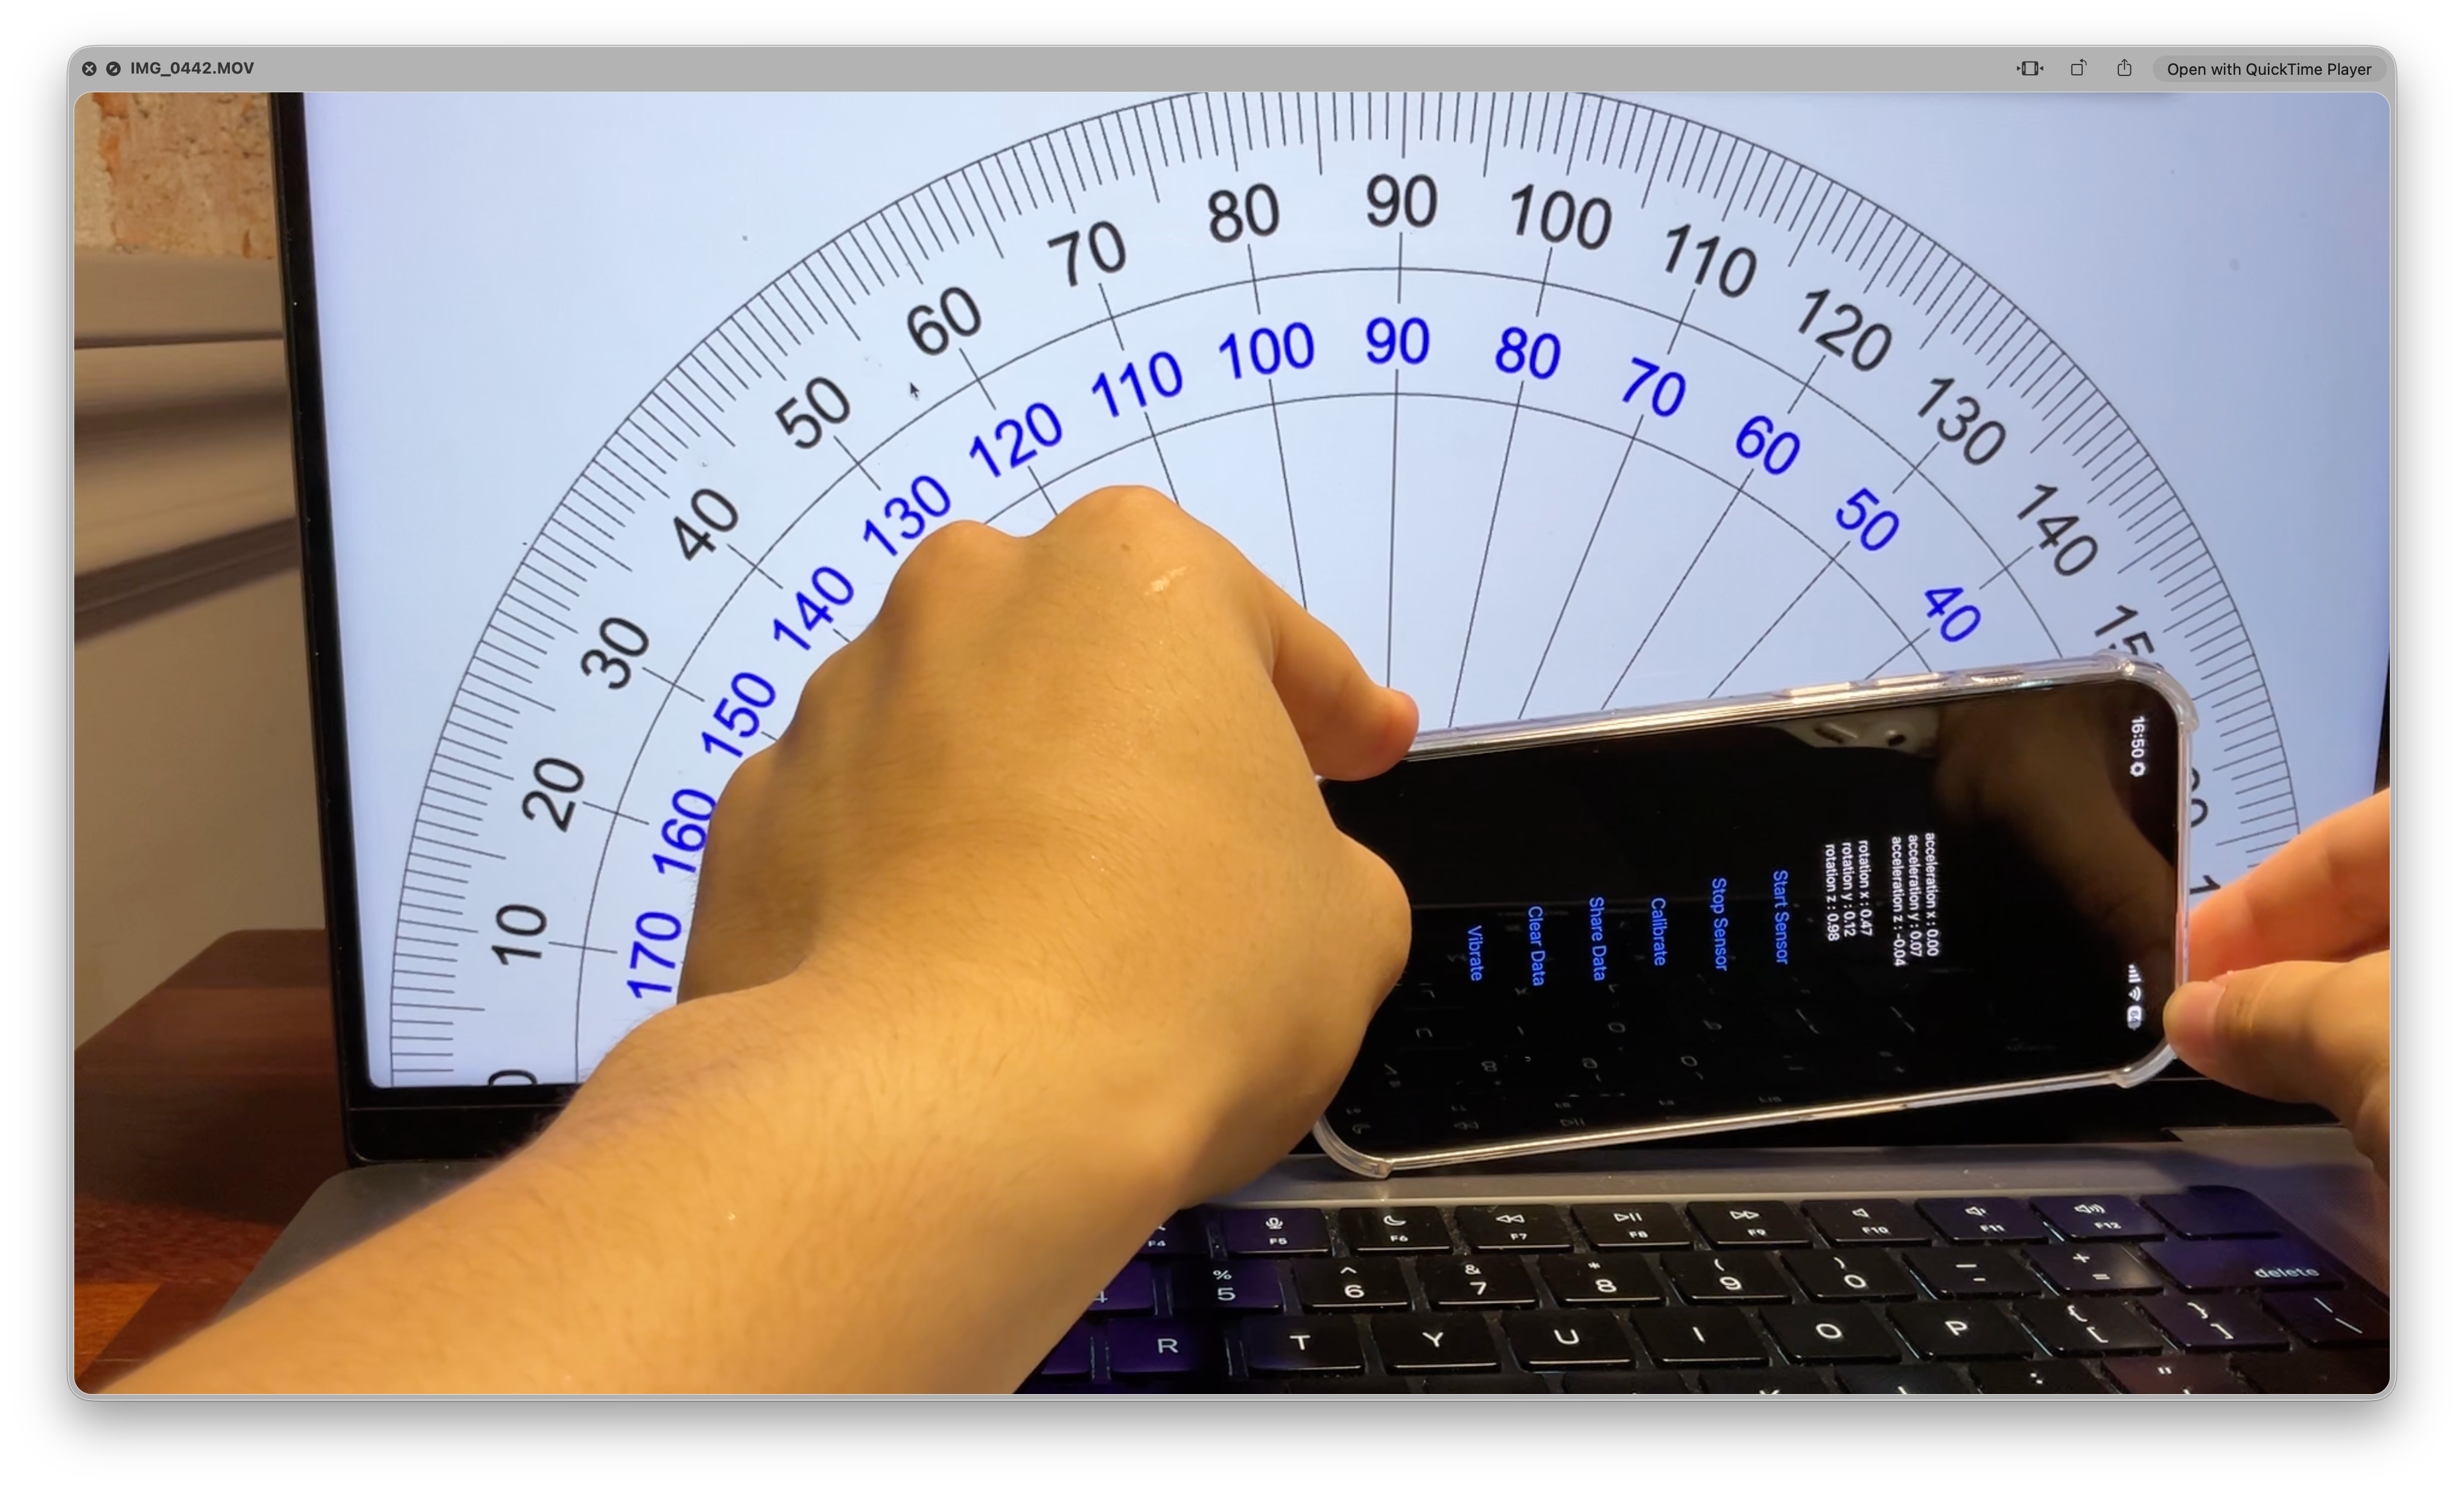
\includegraphics[width=0.9\textwidth]{Images/2_1_3_2.jpg}
            \caption{Inapposite $\theta_{x}$ caused by $y$, $z$ getting small}
            \label{fig:2_1_3_2}
        \end{subfigure}
        \begin{subfigure}
            {0.48\textwidth}
            \centering
            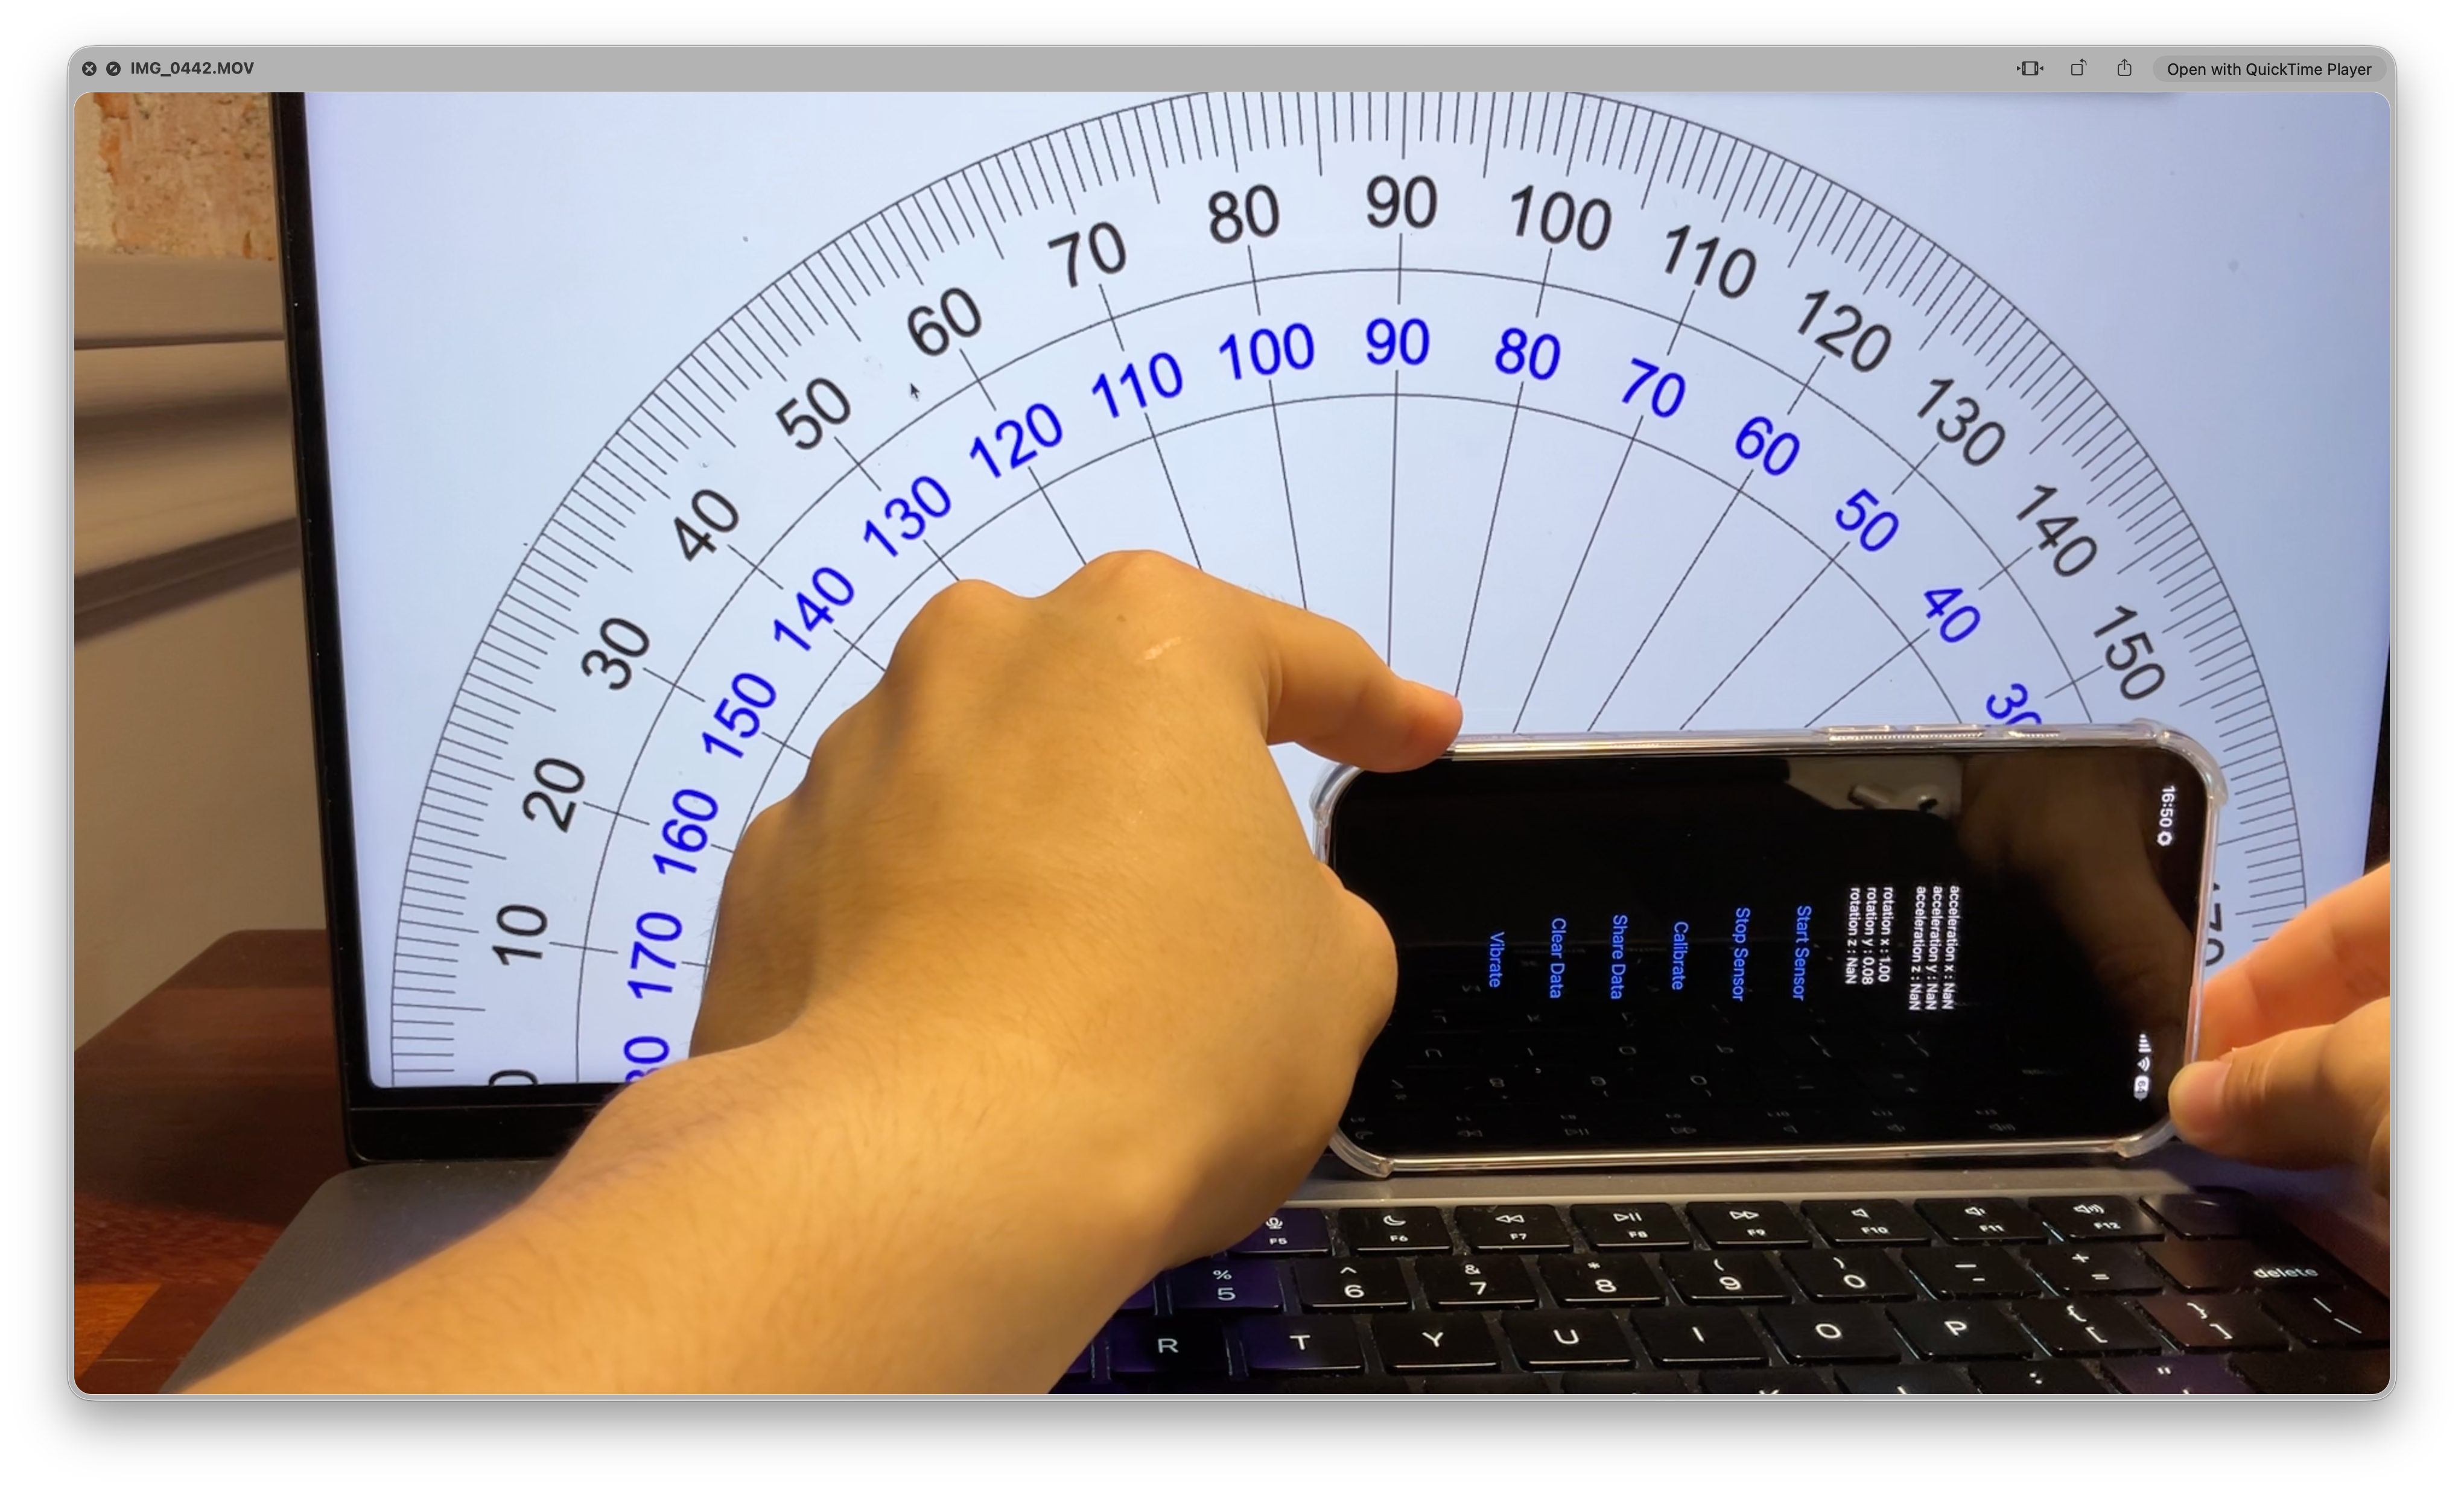
\includegraphics[width=0.9\textwidth]{Images/2_1_3_3.jpg}
            \caption{Error caused by zero $\theta_{x}$}
            \label{fig:2_1_3_3}
        \end{subfigure}
        \begin{subfigure}
            {0.48\textwidth}
            \centering
            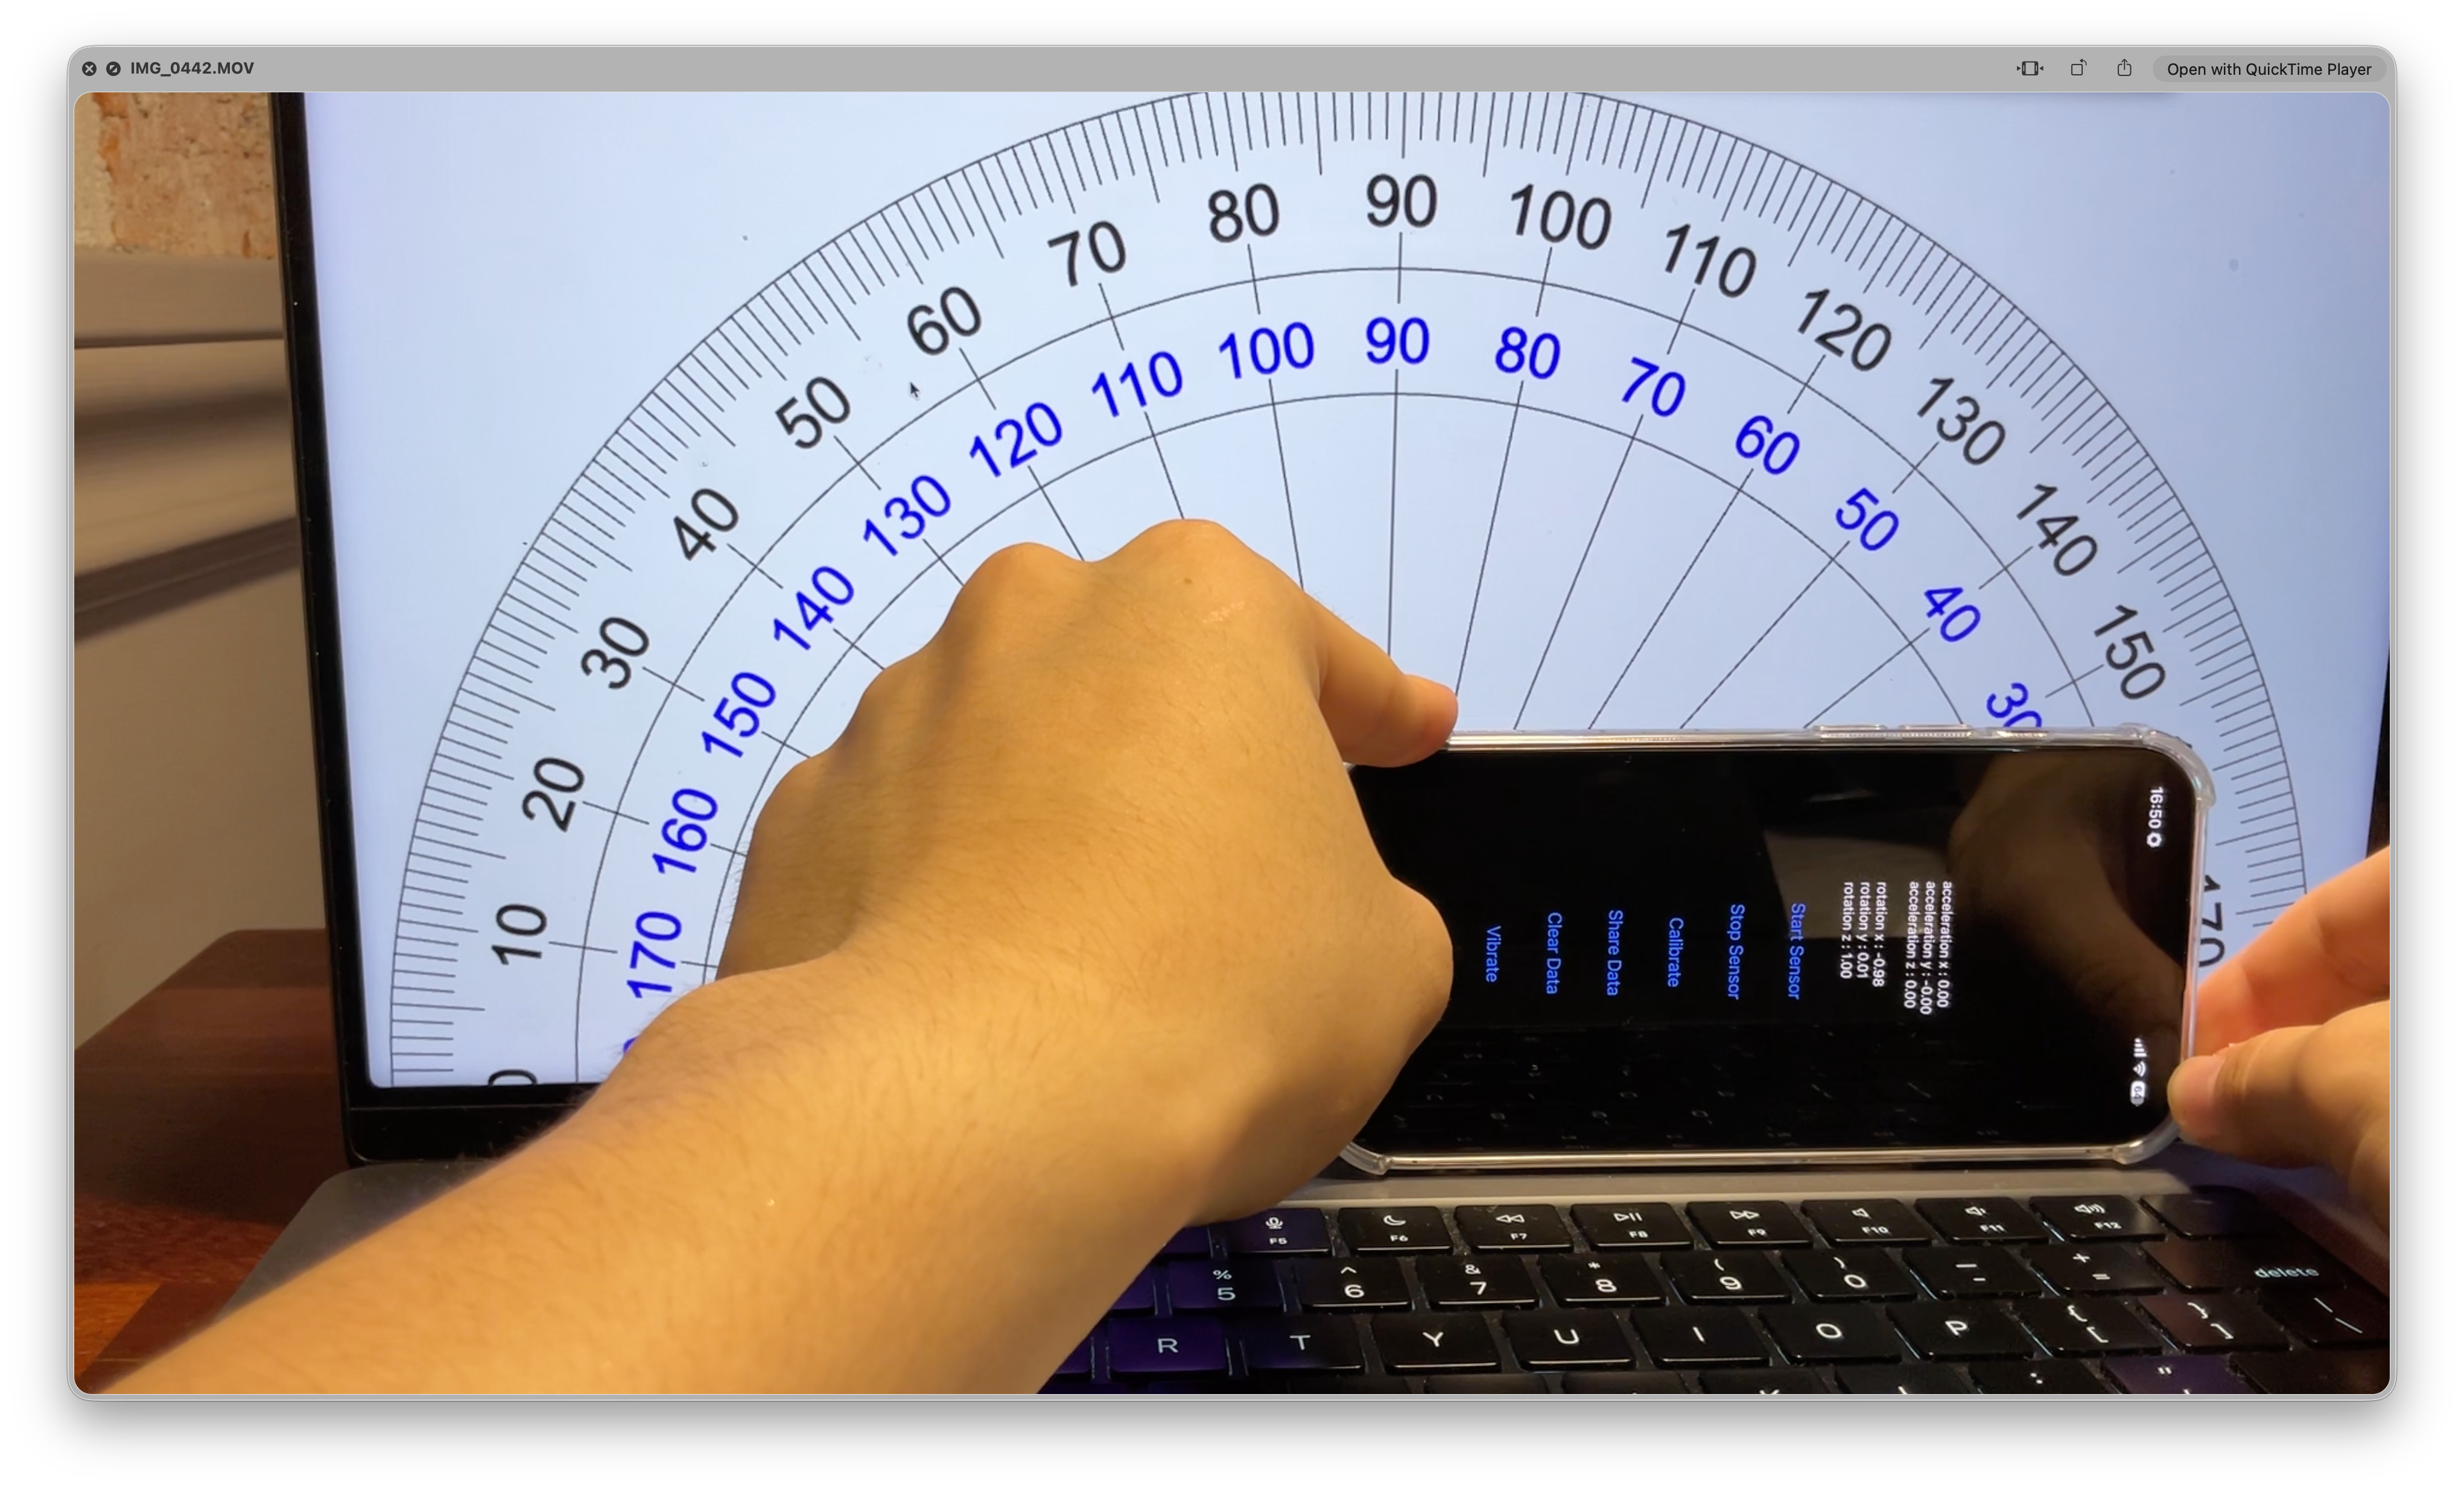
\includegraphics[width=0.9\textwidth]{Images/2_1_3_4.jpg}
            \caption{Inapposite $\theta_{x}$ caused by $y$ to zero}
            \label{fig:2_1_3_4}
        \end{subfigure}
        \caption{A set of images to find the limit of appropriate estimation of
        orientation}
        \label{fig:valid_range_test}
    \end{figure}

    \subsubsection{Orientation Tracking Using the Gyroscope}

    To continuously track changes in the smartphone’s orientation during movement,
    we numerically integrated the gyroscope data over time. The trapezoidal rule
    was employed for numerical integration to accumulate angular velocity into angular
    displacement.

    Let $t$ denote the current time, and $\delta t$ the time step between
    measurements. The gyroscope readings collected up to time $t$ are represented
    as:

    \[
        \left[
        \begin{bmatrix}
            x_{0} \\
            y_{0} \\
            z_{0}
        \end{bmatrix},
        \begin{bmatrix}
            x_{\delta t} \\
            y_{\delta t} \\
            z_{\delta t}
        \end{bmatrix}, \cdots,
        \begin{bmatrix}
            x_{t-\delta t} \\
            y_{t-\delta t} \\
            z_{t-\delta t}
        \end{bmatrix},
        \begin{bmatrix}
            x_{t} \\
            y_{t} \\
            z_{t}
        \end{bmatrix}
        \right]
    \]

    The orientation of the smartphone at each corresponding time step is given
    by:

    \[
        \left[
        \begin{bmatrix}
            \psi_{0}   \\
            \theta_{0} \\
            \phi_{0}
        \end{bmatrix},
        \begin{bmatrix}
            \psi_{\delta t}   \\
            \theta_{\delta t} \\
            \phi_{\delta t}
        \end{bmatrix}, \cdots,
        \begin{bmatrix}
            \psi_{t-\delta t}   \\
            \theta_{t-\delta t} \\
            \phi_{t-\delta t}
        \end{bmatrix},
        \begin{bmatrix}
            \psi_{t}   \\
            \theta_{t} \\
            \phi_{t}
        \end{bmatrix}
        \right]
    \]

    Here, the initial gyroscope reading $\begin{bmatrix}
        x_{0} & y_{0} & z_{0}
    \end{bmatrix}^{\top}$ is assumed to be zero, and the initial orientation $\begin{bmatrix}
        \psi_{0} & \theta_{0} & \phi_{0}
    \end{bmatrix}^{\top}$ is taken from the accelerometer-based estimation described
    in Section~2.1.2.

    To compute the current orientation $\begin{bmatrix}
        \psi_{t} & \theta_{t} & \phi_{t}
    \end{bmatrix}^{\top}$, we use the trapezoidal integration method:

    \[
        \psi_{t}= \frac{1}{2}(x_{t}+ x_{t - \delta t}) \cdot \delta t + \psi_{t
        - \delta t}
    \]
    \[
        \theta_{t}= \frac{1}{2}(y_{t}+ y_{t - \delta t}) \cdot \delta t + \theta_{t
        - \delta t}
    \]
    \[
        \phi_{t}= \frac{1}{2}(z_{t}+ z_{t - \delta t}) \cdot \delta t + \phi_{t
        - \delta t}
    \]

    Through this integration, the angular velocity data from the gyroscope can be
    accumulated to track the smartphone’s orientation over time.

    \FloatBarrier
    \begin{figure}[ht]
        \centering
        \includegraphics[width=\textwidth]{2_1_4_1.png}
        \caption{Orientation tracking using trapezoidal integration of gyroscope
        data}
        \label{fig:gyro_integration}
    \end{figure}

    \FloatBarrier
    \subsubsection{Removal of the Gravity Component}

    The smartphone's accelerometer inherently includes the effect of gravity. To
    isolate the linear acceleration resulting purely from the device’s movement,
    the gravitational component must be removed. This is accomplished by
    reconstructing the gravity vector using the orientation estimated in the
    previous steps.

    This process is essentially the inverse of the approach described in Section~2.1.2.
    When the device is held vertically with its screen facing the user, the expected
    acceleration due to gravity is $\vec{g}$. By rotating this reference vector
    according to the current orientation of the device, we can recover the instantaneous
    gravity vector in the device's coordinate frame.

    Let the current orientation of the device be represented by the Euler angles:

    \[
        \begin{bmatrix}
            \psi_{t}   \\
            \theta_{t} \\
            \phi_{t}
        \end{bmatrix}
    \]

    and let the reconstructed gravity vector at time $t$ be denoted as 3-dimensional
    vector $\vec{g}_{t}$. Then, the gravity vector is given by:

    \[
        \vec{g}_{t}=
        \begin{bmatrix}
            -\sin\phi_{t}             \\
            -\cos\psi_{t}\cos\phi_{t} \\
            \sin\psi_{t}\cos\phi_{t}
        \end{bmatrix}
    \]

    Finally, the linear acceleration $\vec{A}_{t}$ caused by the actual movement
    of the device can be extracted by subtracting the gravity vector from the
    raw accelerometer reading $\vec{a}_{t}$:

    \[
        \vec{A}_{t}= \vec{a}_{t}- \vec{g}_{t}
    \]

    This process enables accurate detection of motion-induced acceleration ignoring
    the gravitational effect in real time.

    \FloatBarrier
    \begin{figure}[ht]
        \centering
        \includegraphics[width=\textwidth]{2_1_5_1.png}
        \caption{Estimated gravity component arranged by time}
        \label{fig:gravity_component}
    \end{figure}
    \FloatBarrier
    \begin{figure}[ht]
        \centering
        \includegraphics[width=\textwidth]{2_1_5_2.png}
        \caption{Comparing between raw data and gravity component removed data}
        \label{fig:removal_of_gravity_component}
    \end{figure}

    \FloatBarrier
    \subsubsection{Auto Calibration of Orientation}
    Since gyroscopes accumulate error over time, the orientation should be periodically
    recalibrated. To achieve this, if the magnitude of the acceleration vector is
    below a certain threshold(which is set to 1.1) and the device is able to
    calibrate its orientation(Section~2.1.3), the orientation is recalibrated through
    the accelerometer data(Section~2.1.2).

    \FloatBarrier
    \begin{figure}[ht]
        \centering
        \includegraphics[width=\textwidth]{auto_calibration_flow_chart.png}
        \caption{Flow chart for the auto calibration process}
        \label{fig:auto_calibration_flow_chart}
    \end{figure}

    \FloatBarrier
    \subsubsection{Noise Removal}
    When estimating position from accelerometer data, numerical integration over
    time often leads to the accumulation of error, resulting in a gradual
    degradation of accuracy. Figure~\ref{fig:integration_drift} illustrates this
    phenomenon.

    In this experiment, the smartphone was placed flat with its $z$-axis
    perpendicular to the ground. A simple up-and-down motion was performed by slowly
    lifting and lowering the device. Theoretically, this movement should result in
    a sinusoidal pattern in the $z$-axis acceleration, ideally resembling a
    function of the form $\sin x,\ x \in [0,\ 2\pi]$.

    However, the actual measurements deviated significantly from this expected pattern.
    As shown in the graph, the $z$-axis acceleration (blue line) did not follow the
    anticipated sine wave. Surprisingly, the $x$-axis—unrelated to the vertical motion—displayed
    unexpected fluctuations, and the $y$-axis exhibited a divergence trend over
    time.

    These anomalies highlight the impact of sensor noise and the sensitivity of
    numerical integration to even minor inaccuracies. Small errors in acceleration
    accumulate rapidly during integration, leading to significant drift in the
    estimated position that does not correspond to the actual motion.

    Therefore, to achieve reliable position tracking, the incorporation of
    advanced noise reduction techniques is essential.

    \FloatBarrier
    \begin{figure}[ht]
        \centering
        \includegraphics[width=\textwidth]{2_1_6_1.png}
        \caption{Aceleration, speed, position data before noise removal}
        \label{fig:integration_drift}
    \end{figure}

    \FloatBarrier
    \subsubsection{Noise Removal - Using Threshold}

    To reduce noise in the accelerometer data, a simple threshold-based filtering
    technique was initially employed. This method assumes that if the difference
    between the current and previous sensor readings is below a predefined
    threshold, the change is not significant and thus the previous value is retained
    instead of updating with the new measurement.

    To determine an appropriate threshold, we analyzed the distribution of
    accelerometer values when the smartphone was stationary, as shown in Figure~\ref{fig:accel_histogram}.
    In this state, the $x$ and $y$ axes—which are not affected by gravity—should
    ideally report values close to zero. However, histogram analysis revealed that
    values commonly fell within the ranges of $0.14$ to $0.15$ and $-0.16$ to $-0
    .15$, indicating the presence of noise rather than actual motion. Based on this
    observation, a threshold of $0.16$ was selected. If the change in acceleration
    between consecutive time steps was less than this threshold, the previous
    value was maintained.

    Despite its simplicity, this method showed limitations in practice.
    Experimental results indicated that the filter failed to capture small but
    meaningful movements and led to accumulated error over time. In other words,
    the threshold-based approach lacked the sensitivity and precision required
    for accurate motion tracking in this study.

    Consequently, we concluded that a more sophisticated filtering technique is necessary.
    We plan to implement the Kalman Filter, a widely used and robust method for dynamic
    state estimation, to improve noise reduction while maintaining
    responsiveness to actual motion.

    \FloatBarrier
    \begin{figure}[ht]
        \centering
        \includegraphics[width=\textwidth]{2_1_7_1.png}
        \caption{Distribution of accelerometer values when the smartphone is
        stationary(each graph shows $x$, $y$, and $z$ axis in order)}
        \label{fig:accel_histogram}
    \end{figure}

    \FloatBarrier
    \subsubsection{Noise Removal - Using Kalman Filter}
    To overcome the limitations of the simple threshold-based noise removal method
    discussed earlier, this study applied a more sophisticated filtering
    technique—the Kalman Filter. The Kalman Filter is widely recognized for its effectiveness
    in noise suppression and state estimation in time-series data, and is
    commonly employed in processing various types of sensor data.

    In this experiment, the Kalman Filter was applied to the accelerometer measurements
    to attenuate sensor noise and achieve more stable position estimation. As
    expected, the filtered output exhibited smoother and more stable transitions
    compared to the previous method, indicating improved noise reduction
    performance.

    However, in terms of positional accuracy, the Kalman Filter did not yield a
    significantly meaningful improvement. While it enhanced the visual smoothness
    of the signal, it was insufficient to correct the inherent drift and
    integration errors associated with accelerometer-based position estimation.

    Therefore, in the next stage of this study, we plan to apply Fast Fourier
    Transform (FFT) techniques to analyze and suppress noise in the frequency
    domain, aiming for further improvement in signal fidelity and positional accuracy.

    \begin{lstlisting}[language=Python, caption={Kalman Filter for noise reduction}, label={lst:kalman_filter}]
acceleration_x = acceleration_x - gravity_x
acceleration_y = acceleration_y - gravity_y
acceleration_z = acceleration_z - gravity_z

kf = KalmanFilter(
    transition_matrices=[1],
    observation_matrices=[1],
    initial_state_mean=0,
    initial_state_covariance=1,
    observation_covariance=1,
    transition_covariance=0.01,
)

state_means_x, state_covariances_x = kf.filter(acceleration_x)
state_means_y, state_covariances_y = kf.filter(acceleration_y)
state_means_z, state_covariances_z = kf.filter(acceleration_z)
\end{lstlisting}

    \FloatBarrier
    \begin{figure}[hp]
        \centering
        \includegraphics[height=0.3\textheight]{2_1_8_1.png}
        \caption{Comparison between raw accelerometer data and noise reduced
        accelerometer data using Kalman Filter}
        \label{fig:accel_kalman}
    \end{figure}
    \FloatBarrier
    \begin{figure}[hp]
        \centering
        \includegraphics[height=0.3\textheight]{2_1_8_2.png}
        \caption{Comparison between raw speed data and noise reduced speed data
        using Kalman Filter}
        \label{fig:speed_kalman}
    \end{figure}
    \FloatBarrier
    \begin{figure}[ht]
        \centering
        \includegraphics[height=0.3\textheight]{2_1_8_3.png}
        \caption{Comparison between raw position data and noise reduced position
        data using Kalman Filter}
        \label{fig:position_kalman}
    \end{figure}

    \FloatBarrier
    \subsubsection{Noise Removal - Using FFT(Fast Fourier Transform)}
    Given the lack of significant improvement in position estimation accuracy after
    applying the Kalman Filter, this study further explored frequency-based
    noise reduction techniques using the Fast Fourier Transform (FFT). FFT is a powerful
    method that converts discrete acceleration signals from the time domain into
    the frequency domain, allowing for the identification and removal of high-frequency
    components or unwanted noise.

    In this experiment, FFT was applied to the time-series accelerometer data to
    obtain its frequency spectrum. Frequency components with amplitudes below a
    threshold of 0.1 were considered insignificant and were eliminated. Subsequently,
    the Inverse FFT (IFFT) was used to reconstruct the denoised signal in the
    time domain.

    Despite the theoretical effectiveness of this approach, the experimental results
    showed no substantial improvement in position estimation accuracy. The
    reconstructed signals appeared cleaner, but the overall trajectory estimation
    remained inaccurate. Thus, the FFT-based filtering approach, like previous
    methods, did not yield a practically meaningful enhancement in performance.
    \begin{lstlisting}[language=Python, caption={Fast Fourier Transform for noise reduction}, label={lst:fft_noise_reduction}]
n = len(fft_time)

fft_x = np.fft.fft(fft_acceleration_x)
fft_x_single = np.abs(fft_x[:n//2])
fft_x_single[1:] = 2 * fft_x_single[1:]

fft_y = np.fft.fft(fft_acceleration_y)
fft_y_single = np.abs(fft_y[:n//2])
fft_y_single[1:] = 2 * fft_y_single[1:]

fft_z = np.fft.fft(fft_acceleration_z)
fft_z_single = np.abs(fft_z[:n//2])
fft_z_single[1:] = 2 * fft_z_single[1:]

frequencies = np.fft.fftfreq(len(fft_time), d=(fft_time[1] - fft_time[0]))
\end{lstlisting}

    \FloatBarrier
    \begin{figure}[ht]
        \centering
        \includegraphics[width=\textwidth]{2_1_9_1.png}
        \caption{Comparision between raw accelerometer data and noise reduced
        accelerometer data using FFT}
        \label{fig:accel_fft}
    \end{figure}
    \FloatBarrier
    \begin{figure}[ht]
        \centering
        \includegraphics[width=\textwidth]{2_1_9_2.png}
        \caption{Comparision between raw speed data and noise reduced speed data
        using FFT}
        \label{fig:speed_fft}
    \end{figure}
    \FloatBarrier
    \begin{figure}[ht]
        \centering
        \includegraphics[width=\textwidth]{2_1_9_3.png}
        \caption{Comparision between raw position data and noise reduced
        position data using FFT}
        \label{fig:position_fft}
    \end{figure}

    \FloatBarrier
    \subsubsection{Limit of Accelerometer}
    Theoretically, integrating acceleration yields velocity, and a second
    integration provides position. However, in real-world environments, this process
    suffers from significant cumulative errors due to the inherent noise present
    in accelerometer measurements. As a result, accurate position estimation using
    raw sensor data becomes extremely challenging.

    To address this issue, several preprocessing techniques were applied, including
    Kalman filtering, Fast Fourier Transformation (FFT), and its inverse. While
    these methods aimed to reduce noise and improve signal quality, they provided
    only marginal improvements in accuracy when considering the limited computational
    resources available on mobile devices. In practice, the increased algorithmic
    complexity outweighed the performance gains, making these approaches less
    suitable for real-time mobile applications.

    In response, this study proposes a novel approach: instead of relying on
    traditional physics-based integration methods, we remove only the gravitational
    component from the acceleration data and employ a deep learning model to learn
    and predict the trajectory of the smartphone. By leveraging data-driven
    learning rather than error-prone numerical integration, this method aims to alleviate
    the issue of accumulated drift and achieve more practical and reliable position
    estimation in mobile environments.

    \subsection{Planning Punch Prediction Model}

    While multiple model architectures were explored—including pure
    Convolutional Neural Networks (CNN) and hybrid CNN-RNN structures—the final
    implementation adopts a lightweight Gated Recurrent Unit (GRU) model. This decision
    is primarily motivated by two factors.

    First, the punch motion exhibits relatively simple and distinct temporal
    patterns that do not require deep spatial feature extraction. Second,
    considering the operational constraints of mobile environments, the model must
    perform inference up to 20 times per second. In this context, the computational
    efficiency of GRU makes it better suited for real-time execution than heavier
    CNN or LSTM-based models.

    Although CNNs and CNN-RNN hybrids (e.g., Conv2D+LSTM or Conv2D+GRU) were evaluated,
    their larger parameter sizes and higher computational cost presented
    challenges for on-device deployment. The GRU architecture, by contrast, achieves
    a good balance between accuracy and speed, especially for time-sensitive
    applications such as punch classification.

    To facilitate faster convergence and enhance model robustness, a \texttt{tanh}
    activation function is applied to the input layer. This serves as a normalization
    step, scaling the accelerometer data to fall within a bounded range, which is
    particularly beneficial when the input magnitude varies significantly across
    different users or punching styles.

    \paragraph{Final GRU-Based Architecture}
    \begin{itemize}
        \item \textbf{Input:} $10 \times 3$ sequence of accelerometer vectors

        \item \textbf{Preprocessing:} \texttt{tanh} activation applied to raw input
            for normalization

        \item \textbf{Recurrent Layer:} Single GRU layer with 8--16 hidden units

        \item \textbf{Fully Connected Layer:} 4 output neurons (for punch classes:
            straight, hook, upper cut, body)

        \item \textbf{SoftMax:} Converts outputs to class probabilities

        \item \textbf{Threshold-Based Trigger:} Inference is executed only when
            the magnitude of acceleration exceeds a predefined threshold
    \end{itemize}

    This design ensures that the model maintains real-time performance with minimal
    energy usage, making it suitable for continuous punch classification on
    mobile devices.

    \subsection{Preparing Punch Dataset}

    \subsubsection{Data Construction}

    To develop an effective deep learning-based punch recognition model, we constructed
    time-series input data derived from smartphone sensor readings and created corresponding
    labeled datasets.

    The raw sensor data were collected using the built-in Inertial Measurement Unit
    (IMU), which includes a 3-axis accelerometer, 3-axis gyroscope, and 3-axis
    magnetometer. However, the magnetometer data were excluded from the model
    due to high noise levels and their limited contribution to motion
    recognition. Similarly, gyroscope data—although useful for orientation
    estimation—were also excluded from the input features to reduce model
    complexity. In contrast, since the x and z axis orientation datas are stable
    and correct in comparison to the y axis, these datas can provide a certain pattern
    for training.

    Based on this setup, the input features $\mathbf{X}$ can be whether
    processed 3-dimension acceleration data or include additional 2 dimensions
    for x, z, axis orientation data over a fixed time window $T$.

    The target label $\mathbf{y}$ corresponds to the punch class annotated at
    each timestamp. The class labels are defined as follows: \texttt{0}: No
    punch detected, \texttt{1}: Straight, \texttt{2}: Hook, \texttt{3}: Uppercut,
    \texttt{4}: Body punch.

    For training, class labels are initially provided as strings (e.g., `"Straight"`,
    `"None"`, etc.), and then encoded either as one-hot vectors for use with the
    \texttt{categorical\_crossentropy} loss function, or as integer indices for \texttt{sparse\_categorical\_crossentropy},
    depending on the model's configuration.

    \begin{lstlisting}[language=Python, caption={Example input-output data format}]
# Example shape: (T, 1, 3)
X = [
    [ acc_x_1, acc_y_1, acc_z_1, (orient_x_1, orient_z_1) ], 
    [ acc_x_2, acc_y_2, acc_z_2, (orient_x_2, orient_z_2) ],
    ...
    [ acc_x_T, acc_y_T, acc_z_T, (orient_x_T, orient_z_T) ]
] # orientation is optional

y = [
  "None",
  "Straight",
  "None",
  ...
  "None",
]
\end{lstlisting}
    This labeling scheme ensures that the model learns not only to recognize punch
    gestures, but also to distinguish them from idle or transitional motion
    patterns. The model is trained to output a class prediction at each time step,
    enabling real-time recognition of punch events as they occur.

    \subsubsection{Data Augmentation Using Sliding Window}

    To increase the size of the training dataset and improve model generalizability,
    we adopted a sliding window algorithm to generate overlapping time-series
    samples. This method is particularly effective for time-dependent sensor data,
    as it allows the model to learn from slightly shifted but semantically
    similar motion sequences.

    Given a raw data stream
    $\mathbf{D}= [\mathbf{d}_{1}, \mathbf{d}_{2}, ..., \mathbf{d}_{n}]$, where each
    $\mathbf{d}_{i}$ is a $3 \times 3$ matrix representing three consecutive accelerometer
    readings across the $x$, $y$, and $z$ axes, we construct input sequences
    $\mathbf{X}$ of fixed length $T$ using a sliding window of size $T$ and
    stride $1$. The label $\mathbf{y}$ for each sequence is assigned based on the
    punch class at the last timestep of the window.

    The following Python snippet illustrates the implementation of this process:

    \begin{lstlisting}[language=Python, caption={Sliding window algorithm for data augmentation}]
WINDOW = 20  # sequence length T

X_list = []
y_list = []

for i in range(len(data) - WINDOW):
    window = data[i:i+WINDOW]
    label = label_list[i + WINDOW - 1]  # label at the last timestep
    X_list.append(window)
    y_list.append(label)
\end{lstlisting}

    This approach enables a significant increase in the number of training
    samples, while preserving the temporal structure of the original data.
    Additionally, by assigning the label based on the final frame in each window,
    the model is encouraged to predict punch classes based on their full
    temporal context, rather than instantaneous changes.

    \subsubsection{Data Accumulation}
    To accumulate the punch dataset, a website was developed to allow users to
    record their punch data using a smartphone. The datas are stored into CloudFlare
    Storage via CloudFlare Workers.

    The columns of the accumulated datasets are as follows:
    \begin{itemize}
        \item \textbf{Index}: The index of the data entry.

        \item \textbf{Time}: The timestamp of the data collection.

        \item \textbf{Raw Acceleration X, Y, Z}: The raw acceleration values recorded
            by the smartphone's accelerometer.

        \item \textbf{Acceleration X, Y, Z}: Gravity-removed acceleration values
            calculated from the raw data.

        \item \textbf{Gyro X, Y, Z}: The gyroscope readings for the x, y, and z axes.

        \item \textbf{Orientation X, Y, Z}: The estimated orientation angles of the
            smartphone in radians.

        \item \textbf{Punch Type}: The type of punch performed, such as "None", "Straight",
            "Hook", "Uppercut", or "Body".
    \end{itemize}

    \FloatBarrier
    \begin{figure}[ht]
        \centering
        \begin{subfigure}
            {0.33\textwidth}
            \centering
            \includegraphics[width=\textwidth]{2_3_3_1.png}
            \label{fig:grip_1}
        \end{subfigure}%
        \begin{subfigure}
            {0.33\textwidth}
            \centering
            \includegraphics[width=\textwidth]{2_3_3_2.png}
            \label{fig:grip_2}
        \end{subfigure}%
        \begin{subfigure}
            {0.33\textwidth}
            \centering
            \includegraphics[width=\textwidth]{2_3_3_3.png}
            \label{fig:grip_3}
        \end{subfigure}
        \caption{A set of images showing the smartphone being held (refer to Figure~\ref{fig:accelerometer}
        for orientation, the dotted lines are negative axes)}
        \label{fig:phone_grips}
    \end{figure}

    \FloatBarrier
    \begin{figure}[ht]
        \centering
        \includegraphics[width=\textwidth]{data_collection_flow_chart.png}
        \caption{Punch data collection website flow chart}
        \label{fig:data_collection_flow_chart}
    \end{figure}
    \FloatBarrier
    \begin{figure}[ht]
        \centering
        \begin{subfigure}
            {0.5\textwidth}
            \centering
            \includegraphics[width=0.35\textwidth]{data_collection_web.png}
            \caption{A screen for recording punch data}
            \label{fig:data_collection_web}
        \end{subfigure}%
        \begin{subfigure}
            {0.5\textwidth}
            \centering
            \includegraphics[width=0.35\textwidth]{data_collection_web_info.png}
            \caption{A screen for viewing recorded punch data}
            \label{fig:data_collection_web_info}
        \end{subfigure}
        \caption{Screenshots of the data collection
        \href{https://punch-boxing.github.io/punch-data-collection-web/}{website}}
        \label{fig:data_collection_web_screenshots}
    \end{figure}

    \FloatBarrier
    \subsection{Analyzing Punch Data}
    As the graph is shown in Figure~\ref{fig:straight_user_input} and Figure~\ref{fig:hook_user_input},
    a Straight punch and a Hook punch seems to have a relation between
    acceleration. Especially the local minima of the X-axis acceleration usually
    matches the peak of the punch. Besides, the value of Y-axis orientation had difference
    with the real situation. This seems to be occured by accumulated error of
    the gyroscope.

    \FloatBarrier
    \begin{figure}[ht]
        \centering
        \includegraphics[width=\textwidth]{straight_user_input.png}
        \caption{Punch data collected from a user performing a straight punch, red
        dots indicate the peak of the punch}
        \label{fig:straight_user_input}
    \end{figure}
    \begin{figure}[ht]
        \centering
        \includegraphics[width=\textwidth]{hook_user_input.png}
        \caption{Punch data collected from a user performing a hook punch, green
        dots indicate the peak of the punch (the y axis orientation is removed
        due to accumulated error)}
        \label{fig:hook_user_input}
    \end{figure}
    \FloatBarrier
    \begin{figure}[ht]
        \centering
        \includegraphics[width=\textwidth]{punch_data.png}
        \caption{Punch data collected from a user performing various punches(straight,
        body, hook, uppercut), each colored dot indicates the punch}
        \label{fig:punch_data}
    \end{figure}

    \FloatBarrier
    \subsection{Building Punch Predict Model}

    Various GRU-based models were built to predict the punch type based on the
    input data. The model architecture is designed to handle time-series data,
    with the input layer accepting sequences of accelerometer readings and the
    output layer predicting the punch class.

    Table~\ref{tab:gru_model_indexing} summarizes the different GRU model
    configurations used in this study. Each model is indexed by its input layer size,
    hidden layer size, number of GRU layers, and window size. The input layer size
    corresponds to the number of features in the input data (e.g., 3 for
    acceleration data, 5 for acceleration data with orientation). The hidden layer
    size determines the number of units in the GRU layer. The window size
    indicates the length of the input sequence used for training. Since a single
    punch can be thrown in a short time, the window size is set to 20, which is equivalent
    to $1(= 0.05 \times 20)$ second. Data used for training is either
    preprocessed acceleration (shown as Acceleration in rest of the paper) data
    or raw acceleration data with orientation.

    \begin{table}[ht]
        \centering
        \begin{tabular}{ |c|c|c|c|c| }
            \hline
            Input Layer Size & Hidden Layer Size & GRU Layer Count & Window Size & Data             \\
            \hline
            3                & 5                 & 1               & 20          & Acceleration     \\
            5                & 10                & 2               &             & Raw Acceleration \\
                             &                   & 4               &             &                  \\
                             &                   & 8               &             &                  \\
            [1ex]             \hline
        \end{tabular}
        \caption{GRU model indexing}
        \label{tab:gru_model_indexing}
    \end{table}

    \begin{center}
        \begin{quote}
            \texttt{GRU\_3I\_5H\_1L\_5W\_A}: GRU model with 3 input features, 5
            hidden units, and 1 layer, trained with acceleration data
            accumulated over a 5 window size
        \end{quote}
    \end{center}

    0.2\% of the total data was used for validation, and early stopping was
    applied with the factor related to the validation loss. Since train data and
    test(validation) data are seperated, the model was trained with the training
    data and evaluated with the validation data.

    In the first try, since it can build a model with fewer code, the model was built
    by TensorFlow and imported to various platforms by TensorFlow.js. However, in
    order to specify options(e.g. adding a hyperbolic tangent layer right behind
    the input layer for data normalization), the model was built again by
    PyTorch. Both codes are available in \href{https://github.com/punch-boxing/punch-ml/}{GitHub}.

    \FloatBarrier
    \subsection{Evaluating Various Punch Predict Model}
    \begin{table}[ht]
        \begin{center}
            \begin{tabular}{ |p{0.45\textwidth}|p{0.45\textwidth}| }
                \hline
                Model Name                        & Validation Accuracy \\
                \hline
                \texttt{GRU\_3I\_5H\_1L\_20W\_A}  & 96.67\%             \\
                \hline
                \texttt{GRU\_3I\_5H\_2L\_20W\_A}  & 97.35\%             \\
                \hline
                \texttt{GRU\_3I\_5H\_4L\_20W\_A}  & 97.59\%             \\
                \hline
                \texttt{GRU\_3I\_5H\_8L\_20W\_A}  & 96.84\%             \\
                \hline
                \texttt{GRU\_3I\_10H\_1L\_20W\_A} & 97.86\%             \\
                \hline
                \texttt{GRU\_3I\_10H\_2L\_20W\_A} & 98.80\%             \\
                \hline
                \texttt{GRU\_3I\_10H\_4L\_20W\_A} & 98.88\%             \\
                \hline
                \texttt{GRU\_3I\_10H\_8L\_20W\_A} & 98.12\%             \\
                \hline
                \texttt{GRU\_3I\_10H\_1L\_20W\_R} & 97.59\%             \\
                \hline
                \texttt{GRU\_3I\_10H\_2L\_20W\_R} & 98.78\%             \\
                \hline
                \texttt{GRU\_3I\_10H\_4L\_20W\_R} & 98.78\%             \\
                \hline
                \texttt{GRU\_3I\_10H\_8L\_20W\_R} & 98.56\%             \\
                \hline
                \texttt{GRU\_5I\_10H\_1L\_20W\_A} & 97.88\%             \\
                \hline
                \texttt{GRU\_5I\_10H\_2L\_20W\_A} & 98.82\%             \\
                \hline
                \texttt{GRU\_5I\_10H\_4L\_20W\_A} & 99.15\%             \\
                \hline
                \texttt{GRU\_5I\_10H\_8L\_20W\_A} & 98.04\%             \\
                \hline
            \end{tabular}
        \end{center}
        \caption{Validation accuracy of various GRU models trained with
        acceleration data}
        \label{tab:gru_model_validation_accuracy}
    \end{table}

    \begin{figure}[ht]
        \centering
        \begin{subfigure}
            {\textwidth}
            \centering
            \includegraphics[width=\textwidth]{GRU_3I_5H_1L_20W_A_GRAPH.png}
            \caption{GRU model with 3 input features, 5 hidden units, and 1
            layer, trained with 20 window size}
            \label{fig:GRU_3I_5H_1L_20W_A_GRAPH}
        \end{subfigure}
        \begin{subfigure}
            {\textwidth}
            \centering
            \includegraphics[width=\textwidth]{GRU_3I_5H_2L_20W_A_GRAPH.png}
            \caption{GRU model with 3 input features, 5 hidden units, and 2
            layers, trained with 20 window size}
            \label{fig:GRU_3I_5H_2L_20W_A_GRAPH}
        \end{subfigure}
        \begin{subfigure}
            {\textwidth}
            \centering
            \includegraphics[width=\textwidth]{GRU_3I_5H_4L_20W_A_GRAPH.png}
            \caption{GRU model with 3 input features, 5 hidden units, and 4
            layers, trained with 20 window size}
            \label{fig:GRU_3I_5H_4L_20W_A_GRAPH}
        \end{subfigure}
        \begin{subfigure}
            {\textwidth}
            \centering
            \includegraphics[width=\textwidth]{GRU_3I_5H_8L_20W_A_GRAPH.png}
            \caption{GRU model with 3 input features, 5 hidden units, and 8
            layers, trained with 20 window size}
            \label{fig:GRU_3I_5H_8L_20W_A_GRAPH}
        \end{subfigure}
        \caption{Various GRU models with different input features, hidden units,
        and layers, trained with acceleration data}
        \label{fig:GRU_3I_5H}
    \end{figure}
    \begin{figure}[ht]
        \centering
        \begin{subfigure}
            {\textwidth}
            \centering
            \includegraphics[width=\textwidth]{GRU_3I_10H_1L_20W_A_GRAPH.png}
            \caption{GRU model with 3 input features, 10 hidden units, and 1
            layer, trained with 20 window size}
            \label{fig:GRU_3I_10H_1L_20W_A_GRAPH}
        \end{subfigure}
        \begin{subfigure}
            {\textwidth}
            \centering
            \includegraphics[width=\textwidth]{GRU_3I_10H_2L_20W_A_GRAPH.png}
            \caption{GRU model with 3 input features, 10 hidden units, and 2
            layers, trained with 20 window size}
            \label{fig:GRU_3I_10H_2L_20W_A_GRAPH}
        \end{subfigure}
        \begin{subfigure}
            {\textwidth}
            \centering
            \includegraphics[width=\textwidth]{GRU_3I_10H_4L_20W_A_GRAPH.png}
            \caption{GRU model with 3 input features, 10 hidden units, and 4
            layers, trained with 20 window size}
            \label{fig:GRU_3I_10H_4L_20W_A_GRAPH}
        \end{subfigure}
        \begin{subfigure}
            {\textwidth}
            \centering
            \includegraphics[width=\textwidth]{GRU_3I_10H_8L_20W_A_GRAPH.png}
            \caption{GRU model with 3 input features, 10 hidden units, and 8
            layers, trained with 20 window size}
            \label{fig:GRU_3I_10H_8L_20W_A_GRAPH}
        \end{subfigure}
        \caption{Various GRU models with different input features, hidden units,
        and layers, trained with acceleration data}
        \label{fig:GRU_3I_10H_A}
    \end{figure}
    \begin{figure}[ht]
        \centering
        \begin{subfigure}
            {\textwidth}
            \centering
            \includegraphics[width=\textwidth]{GRU_3I_10H_1L_20W_R_GRAPH.png}
            \caption{GRU model with 3 input features, 10 hidden units, and 1
            layer, trained with 20 window size}
            \label{fig:GRU_3I_10H_1L_20W_R_GRAPH}
        \end{subfigure}
        \begin{subfigure}
            {\textwidth}
            \centering
            \includegraphics[width=\textwidth]{GRU_3I_10H_2L_20W_R_GRAPH.png}
            \caption{GRU model with 3 input features, 10 hidden units, and 2
            layers, trained with 20 window size}
            \label{fig:GRU_3I_10H_2L_20W_R_GRAPH}
        \end{subfigure}
        \begin{subfigure}
            {\textwidth}
            \centering
            \includegraphics[width=\textwidth]{GRU_3I_10H_4L_20W_R_GRAPH.png}
            \caption{GRU model with 3 input features, 10 hidden units, and 4
            layers, trained with 20 window size}
            \label{fig:GRU_3I_10H_4L_20W_R_GRAPH}
        \end{subfigure}
        \begin{subfigure}
            {\textwidth}
            \centering
            \includegraphics[width=\textwidth]{GRU_3I_10H_8L_20W_R_GRAPH.png}
            \caption{GRU model with 3 input features, 10 hidden units, and 8
            layers, trained with 20 window size}
            \label{fig:GRU_3I_10H_8L_20W_R_GRAPH}
        \end{subfigure}
        \caption{Various GRU models with different input features, hidden units,
        and layers, trained with raw acceleration data}
        \label{fig:GRU_3I_10H_R}
    \end{figure}
    \begin{figure}[ht]
        \centering
        \begin{subfigure}
            {\textwidth}
            \centering
            \includegraphics[width=\textwidth]{GRU_5I_10H_1L_20W_A_GRAPH.png}
            \caption{GRU model with 5 input features, 10 hidden units, and 1
            layer, trained with 20 window size}
            \label{fig:GRU_5I_10H_1L_20W_A_GRAPH}
        \end{subfigure}
        \begin{subfigure}
            {\textwidth}
            \centering
            \includegraphics[width=\textwidth]{GRU_5I_10H_2L_20W_A_GRAPH.png}
            \caption{GRU model with 5 input features, 10 hidden units, and 2
            layers, trained with 20 window size}
            \label{fig:GRU_5I_10H_2L_20W_A_GRAPH}
        \end{subfigure}
        \begin{subfigure}
            {\textwidth}
            \centering
            \includegraphics[width=\textwidth]{GRU_5I_10H_4L_20W_A_GRAPH.png}
            \caption{GRU model with 5 input features, 10 hidden units, and 4
            layers, trained with 20 window size}
            \label{fig:GRU_5I_10H_4L_20W_A_GRAPH}
        \end{subfigure}
        \begin{subfigure}
            {\textwidth}
            \centering
            \includegraphics[width=\textwidth]{GRU_5I_10H_8L_20W_A_GRAPH.png}
            \caption{GRU model with 5 input features, 10 hidden units, and 8
            layers, trained with 20 window size}
            \label{fig:GRU_5I_10H_8L_20W_A_GRAPH}
        \end{subfigure}
        \caption{Various GRU models with different input features, hidden units,
        and layers, trained with acceleration(x, y, z) and orientation(only x, z)
        data}
        \label{fig:GRU_5I_10H}
    \end{figure}

    \FloatBarrier
    \begin{itemize}
        \item \textbf{Impact of Orientation Data}: Regarding situations represented
            in Figure~\ref{fig:GRU_3I_10H_A}, and Figure~\ref{fig:GRU_5I_10H}, the
            model with 3 input features achieved an average validation accuracy of
            98.415\%, while the model with 5 input features achieved an average validation
            accuracy of 98.4725\%. This suggests that the additional orientation
            data (x, z axes) does not have a significant impact on providing
            useful information for punch classification.

        \item \textbf{Impact of Hidden Layer Size}: Regarding situations represented
            in Figure~\ref{fig:GRU_3I_5H}, Figure~\ref{fig:GRU_3I_10H_A}, models
            with 10 hidden units showed an average validation accuracy of 98.415\%,
            which is slightly higher than models with 5 hidden units resulting in
            an average validation accuracy of 97.1125\%. This indicates that increasing
            the number of hidden units can lead to better validation accuracy than
            models with 5 hidden units.

        \item \textbf{Impact of Number of Layers}: Regarding situations represented
            in Figure~\ref{fig:GRU_3I_5H}, Figure~\ref{fig:GRU_3I_10H_A}, Figure~\ref{fig:GRU_3I_10H_R}
            and Figure~\ref{fig:GRU_5I_10H}, models with 4 layers achieved the
            highest average validation accuracy of 98.6\% compared to models with
            1 layer (97.5\%), 2 layers (98.4375\%) and 8 layers (97.89\%). This
            indicates that increasing the number of layers can lead to better
            validation accuracy, but the performance gain is marginal beyond 4 layers.

        \item \textbf{Impact of Preprocessed Acceleration Data}: Regarding situations
            represented in Figure~\ref{fig:GRU_3I_10H_A}, Figure~\ref{fig:GRU_3I_10H_R},
            models using preprocessed acceleration data showed an average validation
            accuracy of 98.415\%, while models using raw acceleration data achieved
            an average validation accuracy of 98.4275\%. This suggests that removing
            the gravity component from the accelerometer data does not have a significant
            impact on improving the model's performance.
    \end{itemize}

    \FloatBarrier
    \subsection{Applying Model}
    The trained model was deployed on a
    \href{https://punch-boxing.github.io/punch-ml-test-web/}{website} and
    implemented in a mobile application. The website allows users to test the model
    with validation data, while the application provides real-time punch
    classification with the smartphone's accelerometer and gyroscope data. \FloatBarrier

    \section{Results}

    While removing the gravity component from the accelerometer data did not lead
    to a significant improvement in model performance, the application of a deep
    learning model for punch classification yielded promising outcomes. The best-performing
    model achieved a validation accuracy of 99.15\% on the punch dataset, demonstrating
    its ability to effectively distinguish between different types of punches based
    solely on smartphone accelerometer data.

    These results highlight the potential of leveraging smartphone sensors for real-time
    motion recognition. In particular, this approach offers a practical solution
    for punch classification in mobile applications, contributing to more
    engaging and active user experiences—potentially addressing issues
    associated with sedentary lifestyles.

    To further enhance model performance and generalizability, future work may explore
    the following directions:
    \begin{itemize}
        \item \textbf{Data Augmentation}: Expanding the dataset by collecting punch
            data from a more diverse range of users and environments, thereby
            improving the model's robustness across different conditions.

        \item \textbf{Time Interval Adjustment}: Modifying the sensor sampling interval
            to better capture the dynamics of phone movement, which may enable
            classification based on the phone’s positional changes during a
            punch.
    \end{itemize}

    \textbf{All the sources of this project are available in
    \href{https://github.com/punch-boxing/}{GitHub}.}
\end{document}